\documentclass[t, pdftex, aspectratio=169]{beamer}  % for 16:9 slides

\usepackage{graphicx}
\graphicspath{{./figs/}}
\DeclareGraphicsExtensions{.pdf,.jpeg,.png, .jpg, .PNG}

\title{Towards a better E2E testing framework}
\author{Lixun Zhang}
\date{\today}


\begin{document}
\frame{\maketitle}

\begin{frame}
  \frametitle{The Problem and History}
  MLIR\#408: FP16 xdlops tolerance too high?
  \begin{itemize}
  \item The tolerance for fp16 tests is set to $15\%$
  \item For other datatypes, the tolerance is set to $0.0001\%$
  \end{itemize}

  PR\#694: Changed verification threshold for fp16 to $0.0001\%$
  \begin{itemize}
  \item All fp16 tests passed in PR CI
  \item Failed in Nightly CI $\Rightarrow$ failures happened in the Random Tests stage
  \end{itemize}

  PR\#696: Bump fp16 tolerance to $25\%$
  \begin{itemize}
  \item We could not even get back to $15\%$
  \item However, later it turned out all tests passed with $10\%$  
  \end{itemize}

  \vskip+2em
  \centering{\large{Why do some fp16 E2E tests fail?}}
\end{frame}

\begin{frame}
  \frametitle{Experiment Setup}

  Sources of configs: tests from auto\_e2e/, e2e\_for\_pr/, and misc\_e2e/
  \begin{itemize}
  \item Tests in e2e\_for\_pr/ are enabled as fixed tests with GPU validation in PR CI
  \item Tests in auto\_e2e/ are set as random tests with CPU validation in the Nightly CI
  \item Tests in auto\_e2e/ and misc\_e2e/ are also set as fixed tests with GPU validation in the Nightly CI
  \end{itemize}

  Settings of the test
  \begin{itemize}
  \item \texttt{-rand} 1: Generate random numbers as inputs
  \item \texttt{-rand\_min} and \texttt{-rand\_max}: choose the range of the random numbers
  \item \texttt{-pv} and \texttt{-pv\_with\_gpu}: choose the validation method
  \item \texttt{-x2}: enable xdlops
  \end{itemize}

  Hardware
  \begin{itemize}
  \item MI100 gfx908 ixt-rack-112
  \item MI200 gfx90a lockhart5
  \end{itemize}
\end{frame}

\begin{frame}
  \frametitle{How to measure the difference between two outputs (val vs. kern)}

  Element wise difference
  \begin{itemize}
  \item Absolute difference $\text{maxAbsDiff} = \max\limits_i(|\text{val}_i - \text{kern}_i|)$
    % \begin{equation}
    %   \text{maxAbsDiff} = \max\limits_i(|\text{val}_i - \text{kern}_i|)\nonumber
    % \end{equation}
  \item Relative difference (ignore zero denominators)
    \begin{equation}
      \text{maxRelDiff} = \max\limits_i(\frac{|\text{val}_i - \text{kern}_i|}{|\text{val}_i|}), \; |\text{val}_i|>0\nonumber
    \end{equation}
  \item Relative difference (ignore small denominators)
    \begin{equation}
      \text{maxRelDiff}_\text{old} = \max\limits_i(\frac{|\text{val}_i - \text{kern}_i|}{|\text{val}_i|}), \; |\text{val}_i|>1\times10^{-3}\nonumber
    \end{equation}
  \item Epsilon difference
    \begin{equation}
      \text{maxEpsilonDiff} = \max\limits_i(\frac{|\text{val}_i - \text{kern}_i|}{\epsilon_{|\text{val}_i|}})\nonumber
    \end{equation}
    where $\epsilon_{|\text{val}_i|}$ is the precision of fp16 numbers around $\text{val}_i$.
  \end{itemize}
  
\end{frame}

\begin{frame}
  \frametitle{How to measure the difference between two outputs (val vs. kern)}
  \vskip+5em
  RMS: the root mean square difference between two data set $A$ and $B$

  \begin{equation}
    \frac{\sqrt{\sum\limits_{i=1}^N(a_i-b_i)^2}}{\sqrt{N}\cdot\max(\max(|a_i|), \max(|b_i|))}\nonumber
  \end{equation}
\end{frame}

\begin{frame}
  \frametitle{Experiment Results and Observations}

  \begin{itemize}
  \item Four random number ranges are chosen:
    \begin{itemize}
    \item r0: [-1, 1]
    \item r1: [-10, 10]
    \item r4: [1, 5]
    \item r5: [5, 10]
    \end{itemize}
  \item Numbers in the following tables are aggregated among all tests for all settings
  \end{itemize}
\end{frame}


\begin{frame}
  \frametitle{Experiment Results and Observations --- Input number magnitude}

  \begin{columns}
    \column{0.4\linewidth}

    \includegraphics[width=2in]{Input_magnitude}
    \column{0.6\linewidth}

    The left table lists aggregated results on MI200
    \begin{itemize}
    \item In general, errors with r1 ([-10, 10]) is larger than that of r0
    \item Exceptions are maxRelDiff and RMS\\
      because the denominators are smaller with r0
    \end{itemize}
  \end{columns}
\end{frame}

\begin{frame}
  \frametitle{Experiment Results and Observations --- Underflow and overflow}

  \begin{columns}
    \column{0.4\linewidth}

    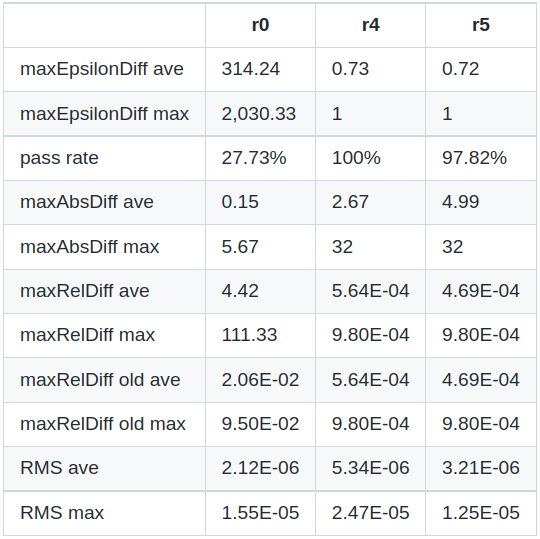
\includegraphics[width=2.3in]{Underflow_overflow}
    \column{0.6\linewidth}

    The left table lists aggregated results on MI200
    \begin{itemize}
    \item In general, errors with r0 ([-1, 1]) is larger than that of r4 ([1, 5]) and r5 ([5, 10])
    \item Exceptions are maxAbsDiff and RMS\\
      because the magnitude of inputs with r4/r5 are lager
    \item A test passes if $\text{maxEpsilonDiff} \le 1$
    \item All tests with r4 pass since the maximum $\text{maxEpsilonDiff}$ is 1
    \item However, some tests with r5 fail even the maximum $\text{maxEpsilonDiff}$ is 1
      $\Rightarrow$ overflow happens
    \end{itemize}
  \end{columns}
\end{frame}

\begin{frame}
  \frametitle{Experiment Results and Observations --- Validation methods}

  \begin{columns}
    \column{0.45\linewidth}

    \includegraphics[width=2.7in]{Validation_method}
    \column{0.55\linewidth}

    The left table lists aggregated results on MI200
    \begin{itemize}
    \item cpu and non-xdlops gpu are closest to each other
    \item cpu and xdlops gpu have medium difference
    \item xdlops gpu and non-xdlops gpu have the largest difference
    \end{itemize}
  \end{columns}

  \vskip+1em
  cpu: sequential implementation of the convolution operation\\
  gpu non-xdlops: convert convolution to gemm and compute gemm without \texttt{mfma}\\
  gpu: convert convolution to gemm and compute gemm with \texttt{mfma}
\end{frame}

\begin{frame}
  \frametitle{Experiment Results and Observations --- MI200 vs. MI100}

  \texttt{mfma} instructions on MI200 flush denormalized numbers to zero
  
  \begin{columns}
    \column{0.7\linewidth}
    
    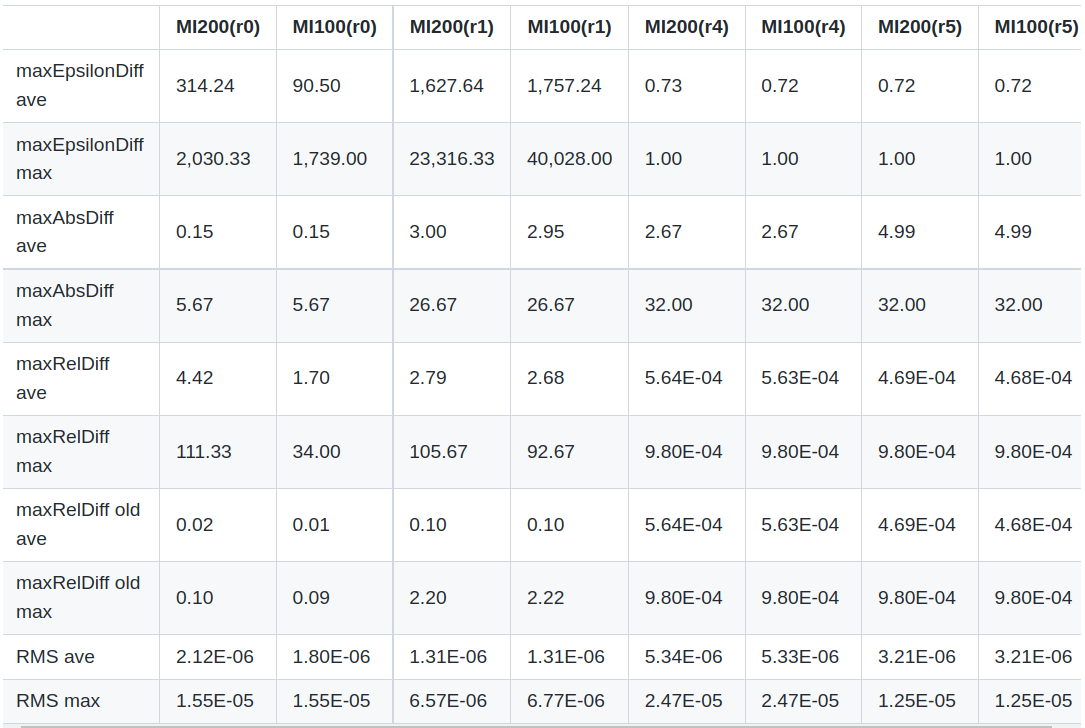
\includegraphics[width=4in]{MI200_MI100}
    
    \column{0.3\linewidth}

    \begin{itemize}
    \item With r4 and r5, MI200 and MI100 behave the same
    \item With r0, MI100 has smaller errors
    \item With r1, MI200 and MI100 behave similarly
    \end{itemize}
  \end{columns}
  
\end{frame}

\begin{frame}
  \frametitle{Experiment Results and Observations --- Exploration of a "better" validation function}
  
  \begin{columns}
    \column{0.5\linewidth}
    
    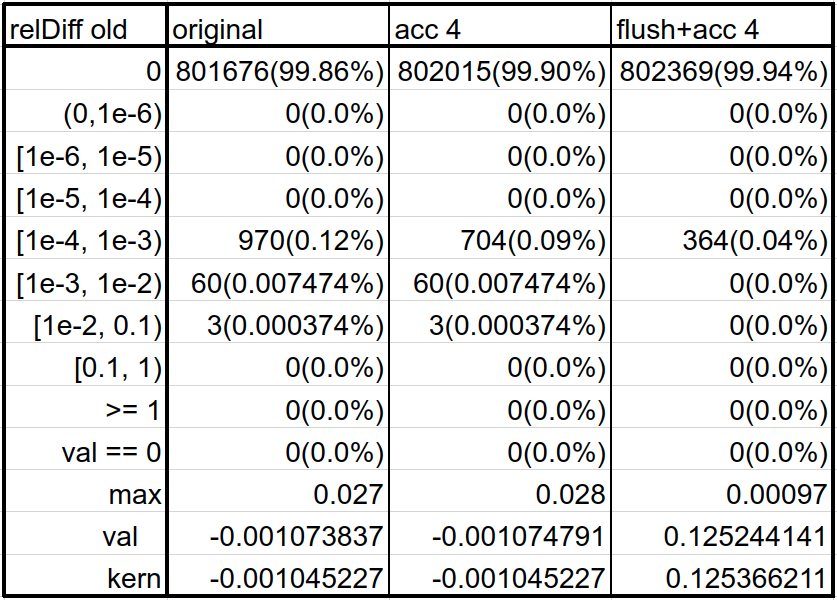
\includegraphics[width=3in]{better_validation}
    
    \column{0.5\linewidth}

    The left table shows the histogram of maxRelDiff\_old of the worst test on MI200
    \begin{itemize}
    \item \texttt{accumulate 4}: cpu truncates the sum of every 4 multiplications from fp64 to fp32
      $\Rightarrow$ slightly improves the results
    \item \texttt{flush subnormals}: cpu flushes small numbers ($<2^{-14}$) to zero
      $\Rightarrow$ greatly improves the results
    \end{itemize}
  \end{columns}
\end{frame}

\begin{frame}
  \frametitle{Summary}

  Causes of numerical errors for fp16 tests:
  \begin{enumerate}
  \item Subnormal numbers flushed to zero
  \item Computation order difference due to partition of gemm onto the grid
  \item Truncation behavior difference during accumulation of intermediate results
  \end{enumerate}
  
  Solutions or workarounds
  \begin{itemize}
  \item Avoid subnormal numbers by choosing a random range away from 0
  \item Use RMS as the metric
  \end{itemize}
\end{frame}

\begin{frame}
  \frametitle{Proposals}
  \begin{enumerate}
  \item MLIR\#620 Apply both RMS and element wise metrics in the verification function
  \item MLIR\#621 Let each test decide how it is passed
    \begin{itemize}
    \item choose which metric to use
    \item choose the tolerance for each metric
    \end{itemize}
  \item MLIR\#619 Auto generate E2E tests at configure or build time
    \begin{itemize}
    \item Organize all configs in the same \texttt{.toml} file
    \item For each config, generate tests for all data types, directions, and layouts.
    \item The MLIR repository only maintains the \texttt{.toml} file and the generation script
      but does not maintain the generated tests.
    \item Stop using fixed tests, all tests use \texttt{-rand 1}
    \item Check all tests in the Nightly CI and select a subset for the PR CI.
      Adjust the metrics and their tolerance based on the selected tests.
    \end{itemize}
  \end{enumerate}
\end{frame}

\end{document}